\subsection{Brainstorming}

In questa fase bisogna farsi venire in mente più idee possibili, focalizzandosi
su:
\begin{itemize}
 \item idea base;
 \item \textit{value proposition};
 \item clienti.
\end{itemize}

Quando si ha un'idea, bisogna segnarsela subito, altrimenti si finisce molto
probabilmente per dimenticarsela. Una volta registrato un insieme di idee, si
può organizzare con l'insieme di persone con cui si vuole iniziare la startup
una sessione di brainstorming.

\paragraph*{Funzionamento di un brainstorming}
Il luogo del brainstorming è importante: deve essere senza continue distrazioni
e non deve bloccare il pensiero creativo. Pensare ad un argomento stando in un
luogo relativo ad esso difatti aumenta la focalizzazione sullo stesso ma
rischia di ``incastrare'' la mente su dei binari di ragionamento predefiniti,
in quanto la nostra mente sarà abituata a ragionare con i metodi di pensiero
tipici del luogo stesso.

Il limite di tempo è utile per mantenere la focalizzazione: questo aumenta la
produttività e riduce le distrazioni. Le idee proposte vanno sempre segnate,
anche se sembrano poco sensate: lo spirito critico va ``spento'' in questo
momento, in quanto non è il contesto adatto.
Una volta pensate le idee vanno selezionate.

Le regole del brainstorming si possono riassumere in:

\begin{itemize}
 \item collocarsi in un ambiente tranquillo, possibilmente con elementi che
rompano la routine;
 \item definire un limite di tempo (ad esempio 1 ora);
 \item focalizzarsi sul tema;
 \item quando qualcuno propone un'idea, cercare a turno di arricchirla;
 \item evitare le critiche, stimolare solo la generazione, non la riduzione;
 \item quando per 2 minuti non si trovano più elementi per arricchire un'idea,
passare alla successiva;
 \item scrivere tutto quello che viene proposto, anche se assurdo.
\end{itemize}

\paragraph*{Selezione delle idee} Dopo la fase generativa si passa alla fase di
ragionamento critico, in cui si passano in rassegna tutte le idee pensate e si
scartano quelle meno sensate. Tra una sessione e l'altra (ovvero tra la
generazione e la selezione delle idee) deve passare un po' di tempo: sessioni
ad una distanza temporale troppo breve danno scarsi risultati.

Lo scopo della selezione è arrivare all'idea migliore tra quelle generate: gli
elementi principali su cui focalizzarsi sono:
\begin{itemize}
 \item l'originalità dell'idea
 \item la sua fattibilità
 \item la passione che essa suscita
\end{itemize}

\subparagraph*{Come eseguire la selezione delle idee} Per selezionare l'idea si
applica la tecnica \textit{kill and thrill}: data un'idea, bisogna trovare
tutti i motivi (in maniera razionale) per cui quell'idea non funzionerebbe e
non sarebbe utile. Dopo aver elencato gli svantaggi, si passa a elencarne tutti
i vantaggi e tutte le motivazioni per cui quell'idea si rivelerebbe vincente.

\noindent Questa metodologia presenta dei rischi:
\begin{itemize}
 \item non riuscire a staccarsi dello status-quo (usare il pensiero laterale!);
 \item farsi spaventare dalle idee coraggiose;
 \item innamorarsi troppo rapidamente di un'idea (non fissarsi sulla prima idea
avuta).
\end{itemize}

\section{Business model, value proposition, USP}

Per ciascuna delle idee selezionate è necessario creare una bozza di business
model. Anche in questo caso è un'attività che coinvolge un'attività di gruppo. È
il momento in cui si crea una bozza su come costituire un'azienda che sia
efficace e sostenibile.

Una startup è un \textbf{progetto di business}, non un'iniziativa di
innovazione.
Un investitore infatti è interessato alla capacità di una startup di
fare business e questo è ciò che ne determina nel medio periodo la
sopravvivenza.

Fare business non significa ottenere i soldi da un investitore. Significa
ottenere un guadagno (sia per lo startupper che per l'investitore) a partire
dai soldi investiti.

Fare business non significa nemmeno avere una base di utenti cospicua: da
sola non basta per reggere in piedi una startup. Occorre generare un guadagno
da tutti gli utenti.

Un business model descrive il modo in cui un'impresa genera valore per i suoi
clienti e \textbf{trasforma questi valori in ricavi}. Aiuta anche a capire:

\begin{itemize}

\item cosa si sta costruendo?

\item cosa serve per costruirlo?

\item a chi si sta proponendo?

\item come trasformare i valori offerti in ricavo?

\end{itemize}

Il business model è un progetto che serve per descrivere ciò che si vuole
compiere. I business model sono spesso degli strumenti che vengono utilizzati
per descrivere i progetti delle startup, in quanto spesso sono facili da capire
e aiutano a descrivere quello che si vuole fare.

Il business model è anche una ``mappa'' che aiuta a guidare verso un obiettivo.
Essa non deve essere fatta solamente dagli startupper, ma può essere utilizzata
anche da aziende. Inoltre, stimola la generazione di nuove idee, evidenziando
possibili novità.

\begin{definition}[Modello di business]
Il \textbf{modello di business} descrive il modo in cui un'organizzazione crea,
distribuisce e cattura valore.
\end{definition}

\subsection{Canvas}

Il canvas serve come strumento per poter rispondere a domande importanti per
capire l'obiettivo e la struttura dell'idea. In particolare, il
canvas si focalizza sui seguenti punti:
\begin{enumerate}
 \item Value proposition: cosa offro ai miei clienti?
 \item Customer segments: chi sono i miei clienti?
 \item Channels: come li raggiungo?
 \item Customer relationship: come curo la relazione con loro?
  \item Key resources: con quali risorse?
 \item Key activities : cosa fa la mia azienda?
 \item Key partners: con che aiuto dall'esterno?
 \item Cost structure: quali sono i costi?
 \item Revenue stream: quali introiti mi porta?
\end{enumerate}

\begin{figure}[t]
 \centering
 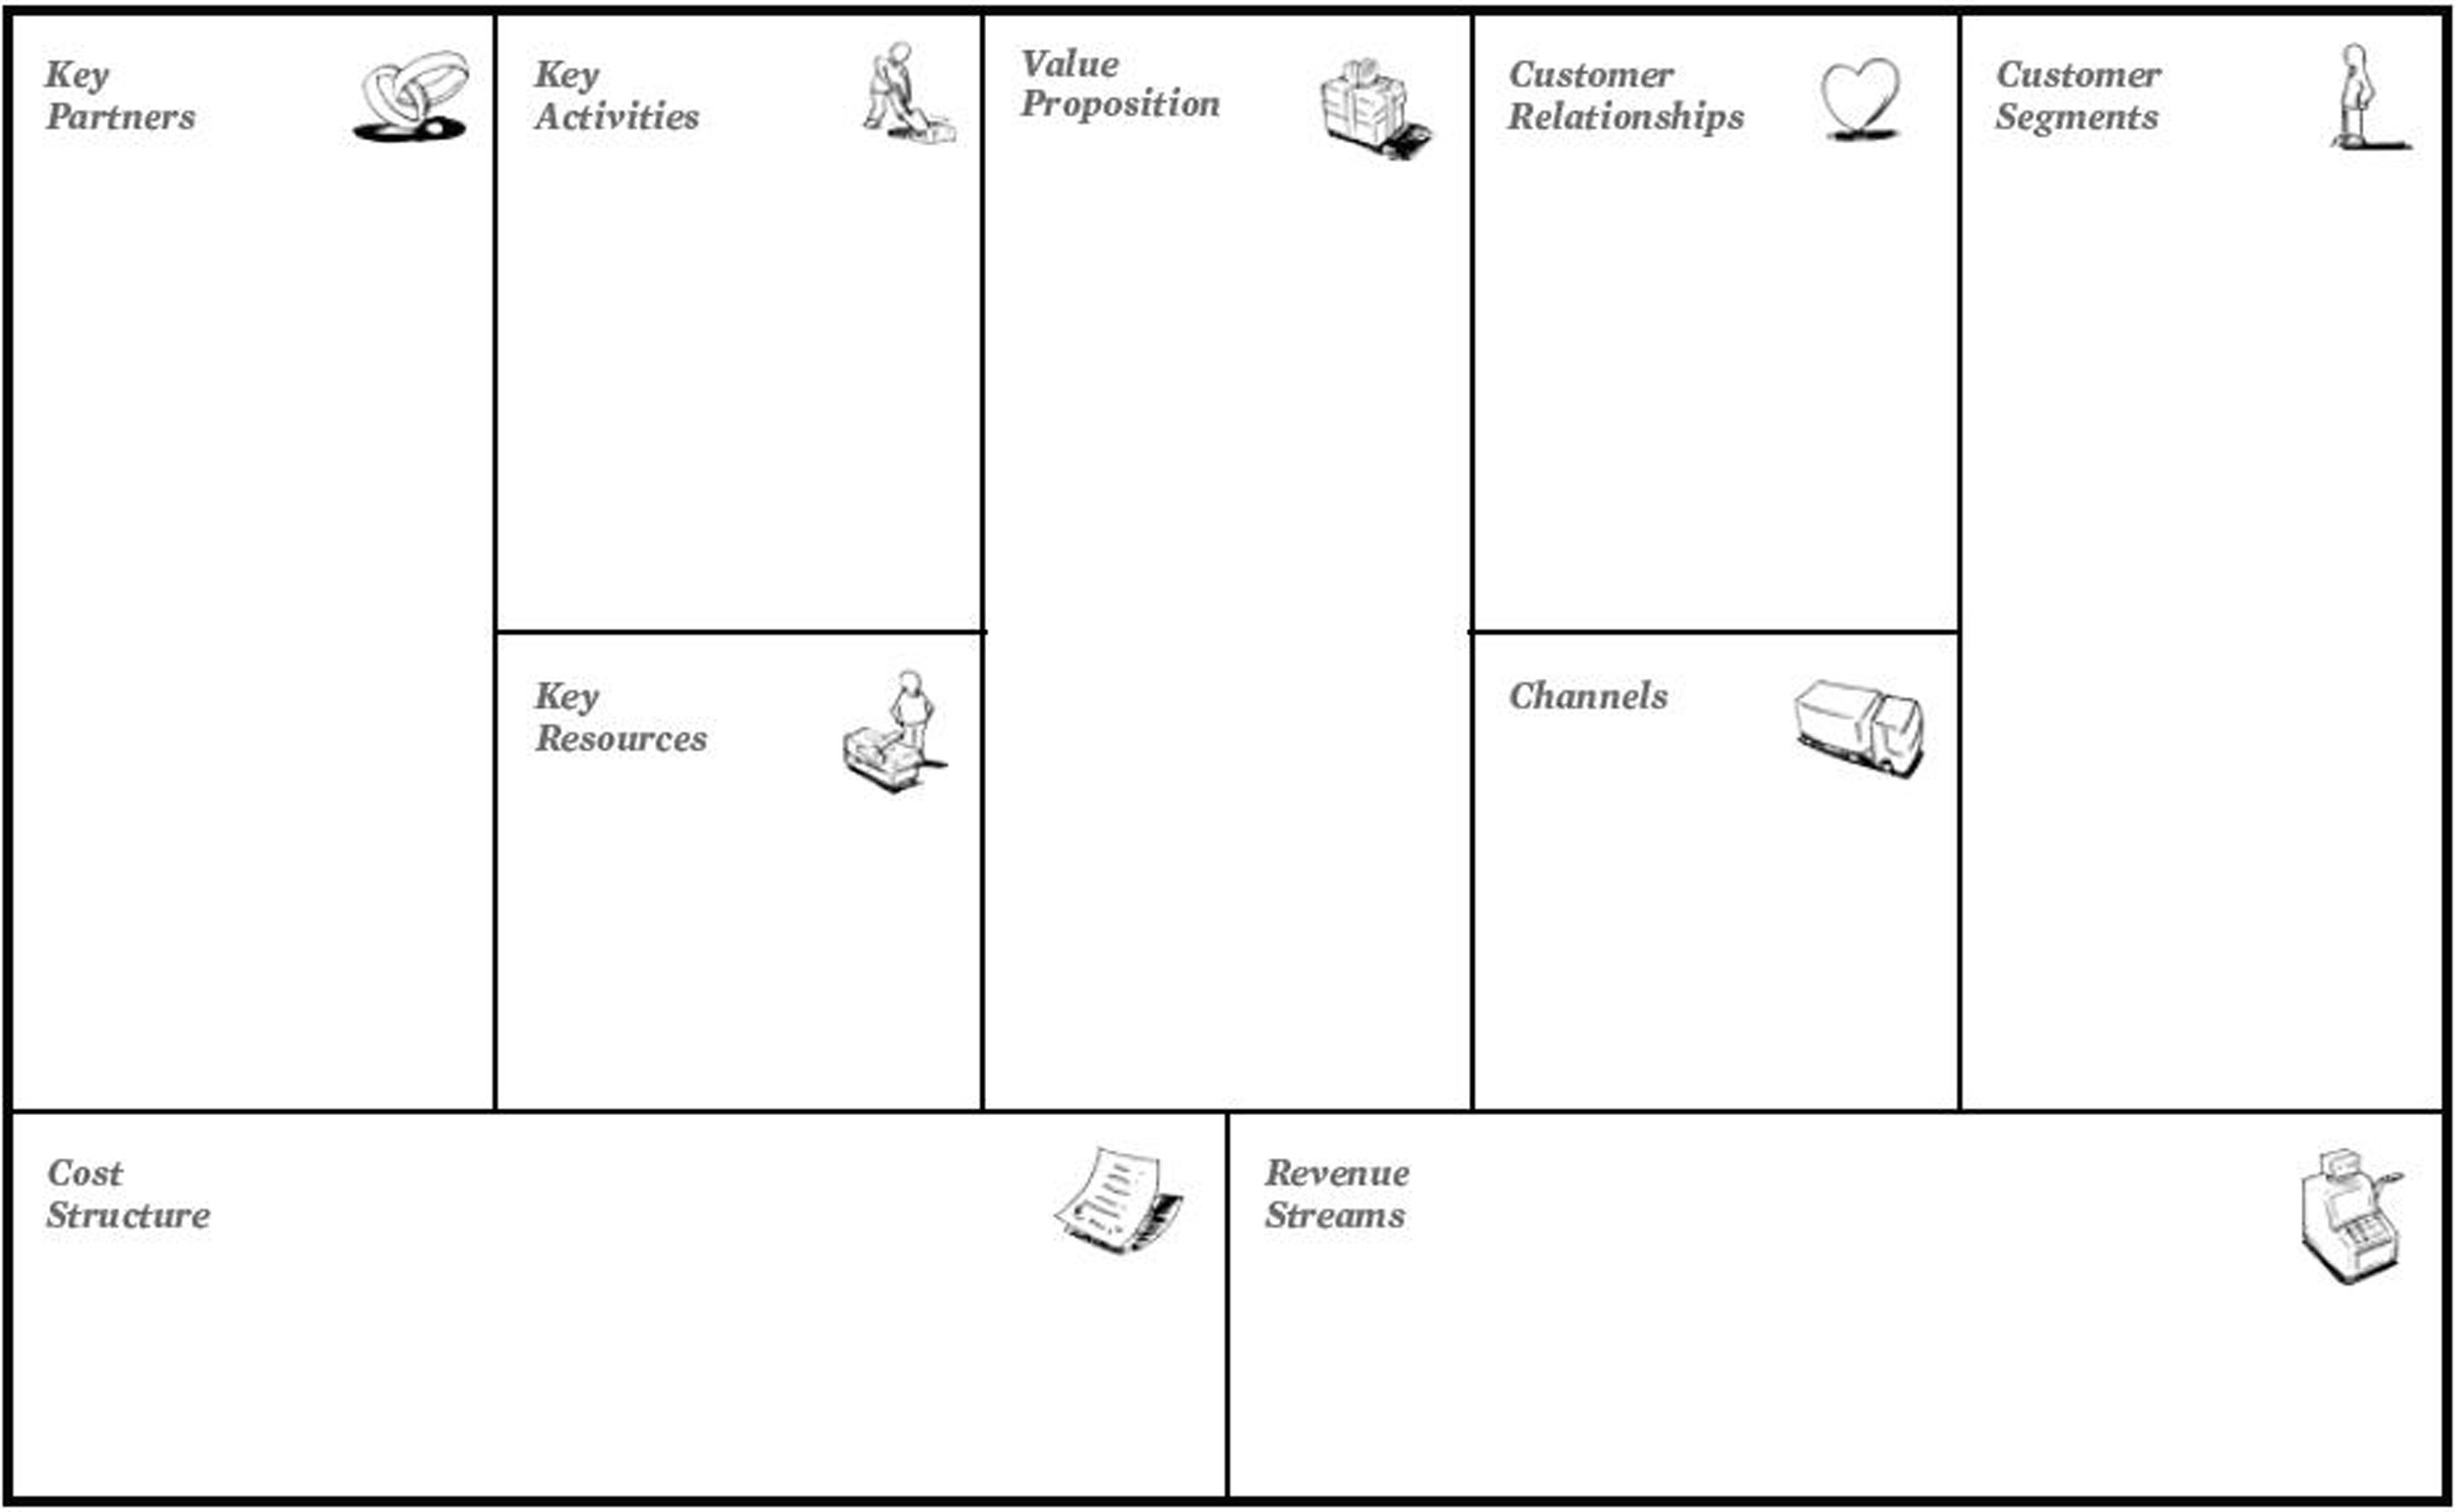
\includegraphics[scale=0.15]{bm_canvas}
 \caption{Canvas di un Business model}
 \label{fig:bm:bm}
\end{figure}

\subsubsection{Value proposition}

\begin{definition}[Value Proposition]
La \textbf{Value Proposition} descrive la serie di prodotti e servizi che
creano valore per il segmento di mercato cui si rivolgono. È un'aggregazione di
benefici che un'organizzazione offre ai suoi clienti.
\end{definition}

Non esistono aziende che non hanno competitors: le aziende che fanno cose
simili, sono, in maniera ovvia, dei competitor tra di loro. Ma non solo:
aziende che producono cose diverse ma soddisfano uno stesso bisogno sono tra di
loro competitors (cioccolateria vs fioraio, Armani vs Ferrari, ecc...).

Nella value proposition ci sono degli elementi chiave, che verranno illustrati
di seguito.

\paragraph*{Novità} Soddisfa un nuovo gruppo di bisogni che precedentemente i
clienti non percepivano come necessari poiché non esisteva un'offerta simile.

Questo non indica un passaggio da un modello di telefono all'altro, piuttosto
il manifestare nuovi bisogni che prima non erano sentiti come necessari.

\paragraph*{Performance} Migliorare un prodotto o un servizio è un metodo
comune per creare valore, come per esempio la crescente potenza di calcolo dei
computer o alla velocità delle auto.

Il miglioramento di performance spesso ha un limite, che è quello percepito
imposto dagli utenti, ad esempio quando la differenza non è abbastanza per
giustificare il prezzo. Oltre a questo, ci sono quelli fisici e legislativi.
